\section{Background Due to Electron Charge Misidentification}
\label{sec:chargeMisID}

After our final event selection, the events are divided into 0SFOS,
1SFOS and 2SFOS channels (where SFOS means same flavor opposite sign
electrons). When an electron charge is mismeasured, a $WZ$ event can
be classified as a 0SFOS event. Electrons that have gone through a
hard bremsstrahlung followed by a photon conversion can have their
charges mismeasured. The effect is negligible for muons.  To estimate
the background with electron charge misidentification, we need to
measure the charge misidentification rates first using \Zee\ events
selected from data. The methods will be described in detail below
starting with the measurement of the charge misID rate, its
uncertainties and its application.

\subsection{Electron charge misidentification}

The electron charge misID rates are measured with data using a
statistical method based on a likelihood. The method is applied on MC
samples and the results are compared with the mischarge rate obtained
using MC truth information. The truth method is applied on \Zee\ MC
samples
(\texttt{mc12\_8TeV.147806.Powheg\\Pythia8\_AU2CT10\_Zee.merge.NTUP\_COMMON.e1169\_s1469\_s1470\_r3542\_r3549\_p1562})
which constitutes a closure test for the likelihood method. Both
methods use events with two good electrons from a $Z$ boson decay. The
events are selected with two good electrons defined by our $WWW$
electron selection with an invariant mass window of ($\mZ - 10\GeV$,
$\mZ + 10\GeV$) where \mZ\ is the PDG $Z$ pole mass of
91.19~\GeV~\cite{PDG:2014}. These events are then divided into same
sign events (SS) and opposite sign events (OS). The mischarge rates
are measured in 2D bins of $\eta$-\pt. The bin boundaries of \pt\ and
$\eta$ are listed in Table~\ref{tab:Etbin and Etabin of mis-charge
  rate}.

\begin{table}[htp]
\centering
\begin{tabular}{c|ccccccccc}
  \hline
  $|\eta|$ bins & [0, 0.8]   & [0.8, 1.15] & [1.15, 1.6] & [1.6, 1.8]
  & [1.8, 2.0]\\
  & [2.0, 2.2]  & [2.2, 2.3]  & [2.3, 2.4] & [2.4, 2.5]  \\
  \hline
  \pt\ bins [\GeV] & [15, 30] & [30, 40] & [40, 50] & [50, 60]
                   & [60, 80] & [80, 120] & [120, 1000]  \\
  \hline
\end{tabular}
\caption{The $\eta$ and \pt\ bins for the measurement of mischarge
  rate.}
\label{tab:Etbin and Etabin of mis-charge rate}
\end{table}


\subsubsection{Truth method and likelihood method}

The truth method is based on the comparison between an electron's true
charge and its reconstructed charge. We still use the \Zee\ MC samples
for the truth measurement. We select two good reconstructed electrons
referred to as ``A'' and ``B'' below with the selection criteria of this
analysis, and find the two truth electrons (referred to as ``C'' and
``D''). To match the reconstructed electrons to the true electrons, we
calculate the $\Delta R = \sqrt{\Delta \eta^2 + \Delta \phi^2}$ of
AC, BD, AD and BC. If $\Delta R$(AC)+$\Delta R$(BD)$\textless$$\Delta
R$(AD)+$\Delta R$(BC), electron A matched with C and B matched with D
otherwise A matched with D and B matched with C. Also, we drop events
with very large $\Delta R $ , $\pt(truth)$ to avoid incorrect
match. Then we compare the charge between the reconstructed electron and
the true electron, counting the number of charge misidentified electrons
and record their $\eta$ and \pt.
  
The likelihood method assumes that for \Zee\ events, the probability
of reconstructing a pair of same sign electrons is ($\varepsilon_1 +
\varepsilon_2$) where $\varepsilon_1$ and $\varepsilon_2$ are the
probabilities of charge misidentification for the two electrons,
respectively. The charge misID rate is parameterized as a function of
$\eta$ and \pt, the $\eta$ dependence is particularly important since
the material distribution (and therefore the conversion rate) is
strongly dependent on the region of the detector where the electron is
reconstructed. The charge misID rates ($\eta$,\pt) are measured from
the total number of events and the number of events with a pair of
same sign electrons by maximizing the following likelihood function
constructed from Poisson statistics: 
\begin{equation}
    \ln\mathcal{L}(\varepsilon|N_{tot},N_{ss}) =
    \sum_{i,j}\ln\left[N_{tot}^{i,j}(\varepsilon_{i}+\varepsilon_{j})\right] N_{SS}^{i,j}-N_{tot}^{i,j}(\varepsilon_{i}+\varepsilon_{j})
    \label{eq:lnL_chargeMisID}
\end{equation}
where $N_{tot}^{i,j}$ and $N_{SS}^{i,j}$ are the total number of
candidate events and the number of which have a same-sign electron
pair, having the first and second lepton in the $i$-th and $j$-th bin
respectively. The bin index $i,j$ denotes each cell in $\eta$-$p_T$ 2D
space.

\subsubsection{Comparison between Likelihood rate and Truth rate}
   The mis-charge rate for $Z\rightarrow ee$ MC sample is measured
   using the likelihood method and is compared with truth mischarge
   rate in Fig.~\ref{fig:LL_Truth_Comparison}.

\begin{figure}[htp]
\centering
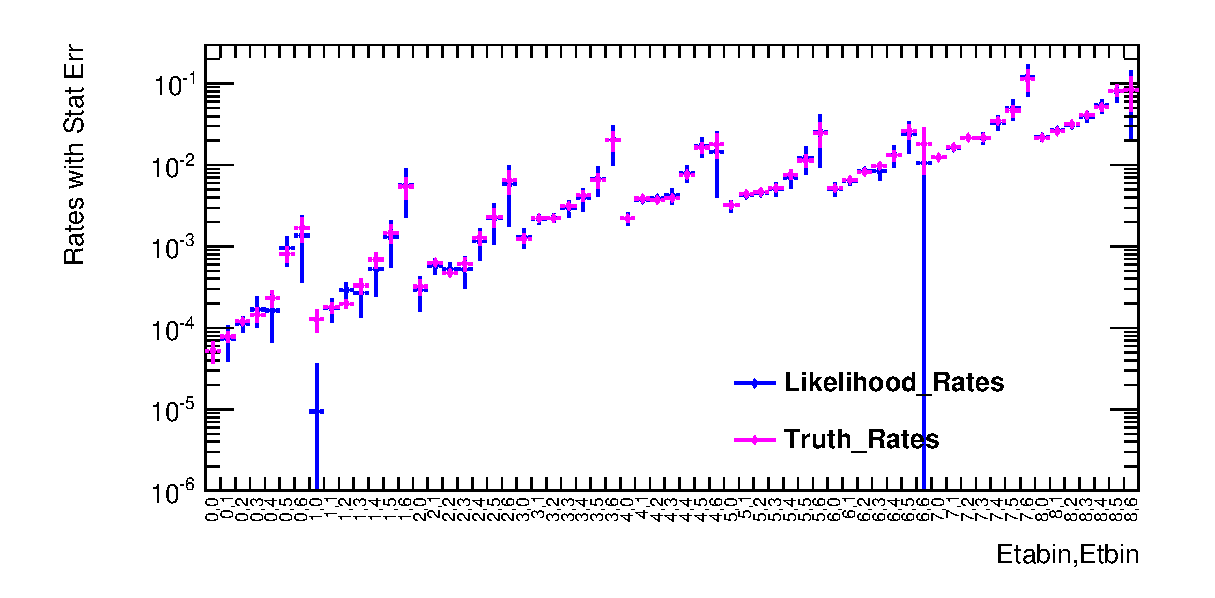
\includegraphics[width=0.8\textwidth]{figures/ChargeMisID/LL_TR_Com.eps}
\caption{This is mis-charge rate comparison between likelihood and
  truth method considering statistic errors. The two sets of rates
  here are both measured with \Zee\ MC samples. The $x$ axis label is
  the \eta, \pt\ bin index.}
\label{fig:LL_Truth_Comparison}
\end{figure}  

Through the comparison, we can see that the rates measured with
likelihood method are compatible with what we measured with truth
method. Using the likelihood method, we measure the mischarge rate
with real data in Egamma stream we measure the data-driven rates with
Egamma
samples(\texttt{user.along528.data12\_8TeV.period*.physics\_EGamma.PhysCont.NTUP\_SMWWW.SMN2N\_2\\Lep\_v1\_EXT0}
where * is A,B,C,D,E,G,H,I,J,L. These samples are slimmed with loose
di-lepton requirement, the di-lepton slim require there are at least 2
tagged high \pt\ leptons where tagged high \pt\ means Electron/Muon
satisfies any object quality requirement (loose, medium or tight for
muons and loose++,\\medium++,tight++,
veryLooseLL,looseLL,mediumLL,tightLL, or veryTightLL for electrons)
and has a pt of at least 10 GeV.). We use the data-driven likelihood
rates as our central values with the effect of background
contamination neglected. We estimate the background effect with
coarser binning and include the shift in mischarge rate in the
systematics.

%  We apply the likelihood method and event selection mentioned before
%  to data and we get the data-driven electron mis-charge rates, but
%  the rates are measured from data so there will be background events
%  remaining in the selected events. We use those rates directly
%  measured from data as central values and then subtract the
%  background contribution in the rates, we can calculate another set
%  of likelihood rates using the events without background, we may
%  call those rates clean rates. The difference between central values
%  and clean rates is the background systematic.

\begin{figure}[htp]
\centering
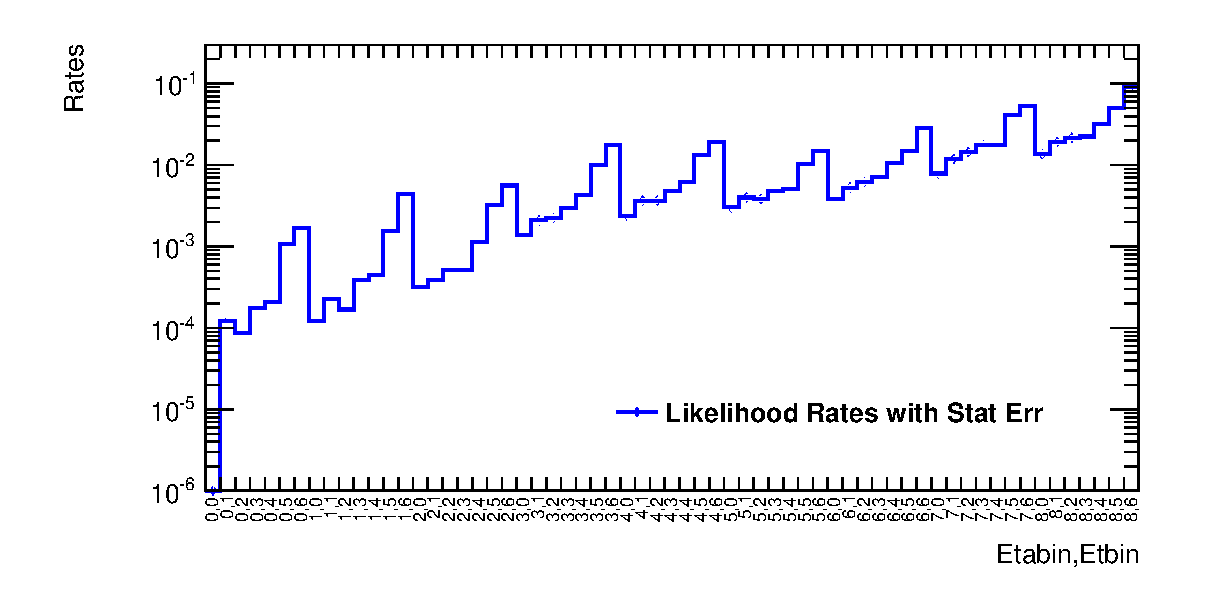
\includegraphics[width=0.8\textwidth]{figures/ChargeMisID/Egamma_LL.eps}
\caption{This is electron mis-charge rates measured from data with likelihood method and its statistic errors. Label on x axis is \eta, \pt\ bin indices.}
\label{fig:LL_Rates_Egamma}
\end{figure}

We use template fit method on the distribution of invariant mass of
the electron pairs to determine the background contribution in total
number of events in each bin ($N^{i,j}_{tot}$ in
Eq.~(\ref{eq:lnL_chargeMisID})) and in number of same sign events in each
bin ($N^{i,j}_{SS}$ in Eq.~(\ref{eq:lnL_chargeMisID})).  We subtract the
estimated background contribution in $N^{i,j}_{SS}$ and
$N^{i,j}_{tot}$ before maximizing the likelihood. This is only
practical with much coarser bins. The signal template is obtained from
\Zee\ MC, and the background template is obtained with data, with some
electron identification and isolation cuts reversed.

\begin{table}
  \centering
  \begin{tabular}{|c|c|}
  \hline
  Signal & Background \\
  \hline
  \texttt{EF\_e24vhi\_medium1} or \texttt{EF\_e60\_medium1} & \texttt{EF\_e24vhi\_medium1} or \texttt{EF\_e60\_medium1} \\
  \hline
  Exactly two electrons passing electron selection & Choose the leading and subleading electrons \\ & and at least one of these 2 electrons \\ & satisfied the background electron selection \\
  \hline
  Trigger Match & \\
  \hline
  $|$ee Invariant Mass - Zmass$|$$\textless$10 GeV & \\
  \hline
  \end{tabular}
\caption{Event selection to select signal and background $ee$ invariant mass histograms.}
\label{tab:Event_Selection}
\end{table}

\begin{table}
  \centering
  \begin{tabular} {|c|c|}
  \hline
  Signal  & Background \\
  \hline
  Author is 1 or 3 & Author is 1 or 3 \\
  \hline
  OQ & OQ \\
  \hline
  $|$\eta$|$ $\textless$ 2.47, crack region removed & $|$\eta$|$ $\textless$ 2.47, crack region removed \\
  \hline
  \pt\ $\textgreater$ 15 GeV & \pt\ $\textgreater$ 15 GeV \\
  \hline
  TightPP & fail TightPP \\
  \hline
  ETcone20/\pt\ $\textless$ 0.10 for \pt\ $\textgreater$ 20GeV & Fail this cut\\ ETcone20/\pt\ $\textless$ 0.07 for \pt\ $\textless$ 20GeV & \\
  \hline
  pTcone20/\pt\ $\textless$ 0.04 & Fail this cut \\
  \hline
  $|$d0/sigmad0$|$$\textless$3.0 & \\
  \hline
  $|$z0*sin(theta)$|$$\textgreater$0.5 & \\
  \hline
  \end{tabular} 
\caption{Electron selection to select signal and background ee
  invariant mass histograms.}
\label{tab:Electron_Selection}
\end{table}

%  With the event and electron selection we can get the signal $ee$ invariant mass histogram from \Zee\ MC samples and background $ee$ invariant mass histogram from data. Because the events are divided into many bins and the statistic will be too low to apply template fit, we will merge the bins of the electrons so that we will get enough statistic to do background subtraction. 
To improve the statistical precision, we merge the $p_T$ bins and then
the events will be divided into $9\times 9$ \eta-bins. We will choose
events with the first electron's $|\eta|$ between [0,0.8] and the
second electron's $|\eta|$ between [1.15,1.60] to illustrate the
procedure. The $ee$ invariant mass distribution obtained from the
\Zee\ MC samples using the background selection (shown in
Table~\ref{tab:Electron_Selection}) is presented in
Fig.~\ref{fig:Mee} (left) and the background $ee$ invariant mass
selected from data using the background selection is presented in
Fig.~\ref{fig:Mee} (right).
 
\begin{figure}[htbp] 
  \centering
  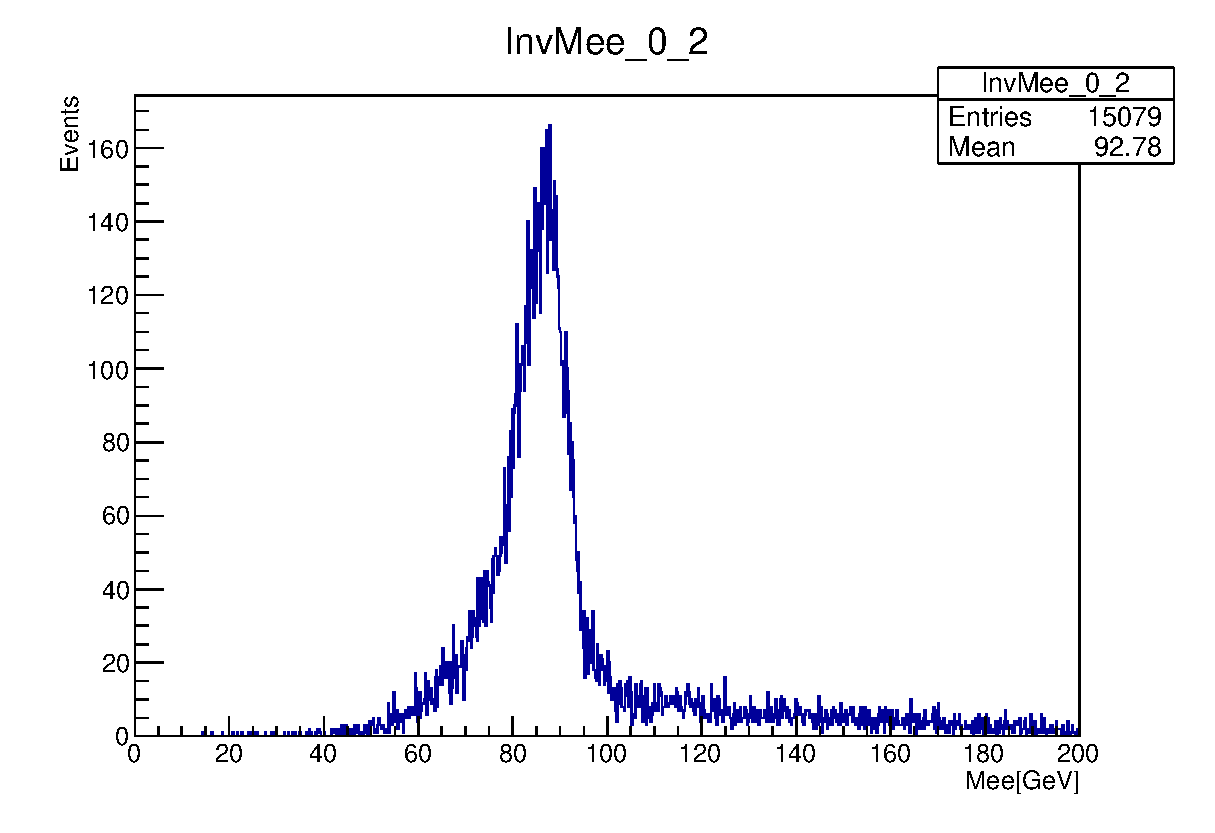
\includegraphics[width=0.49\textwidth]{figures/ChargeMisID/MergeEt_Ntot_ZeeBkg02.eps}
  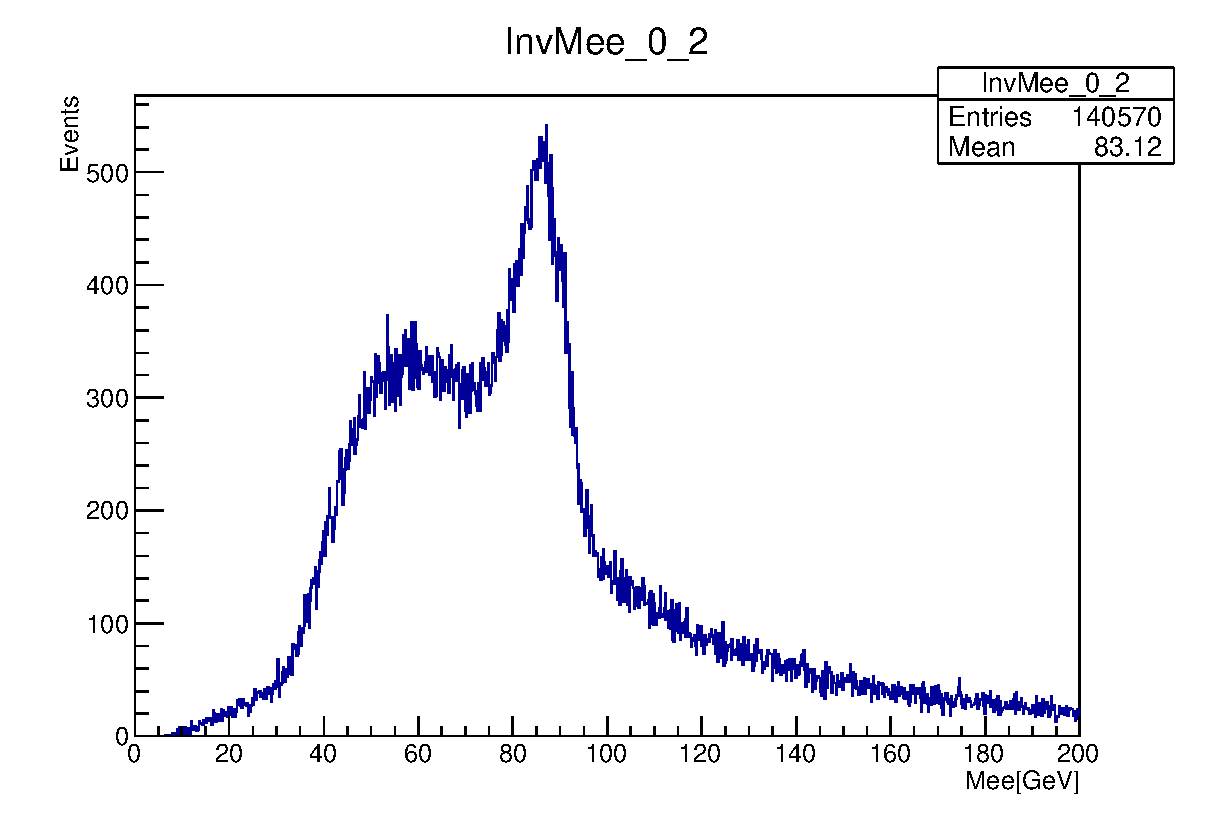
\includegraphics[width=0.49\textwidth]{figures/ChargeMisID/MergeEt_Ntot_Bkg02.eps}
  \caption{The $ee$ invariant mass obtained from \Zee\ MC samples
    (left) and from data (right) using the background selection in
    Table~\ref{tab:Electron_Selection} and
    Table~\ref{tab:Event_Selection}.}
  \label{fig:Mee}
\end{figure}

 We can see that the signal $ee$ invariant mass histogram looks fine
 but for the background $ee$ invariant mass histogram, there is an
 obvious peak around $Z$ mass area which is because there are
 \Zee\ events remaining in the background histogram. We fit the $ee$
 invariant mass spectrum with signal template obtained from MC and a
 polynomial function to describe the background. The polynomial
 function obtained in the fit is then used as the background
 template. The polynomial fit for events with first electron's
 $|\eta|$ between [0,0.8] and second electron's $|\eta|$ between
 [1.15,1.60] is shown in Fig.~\ref{fig:Polynomialac}.
\begin{figure}[htp]
\centering
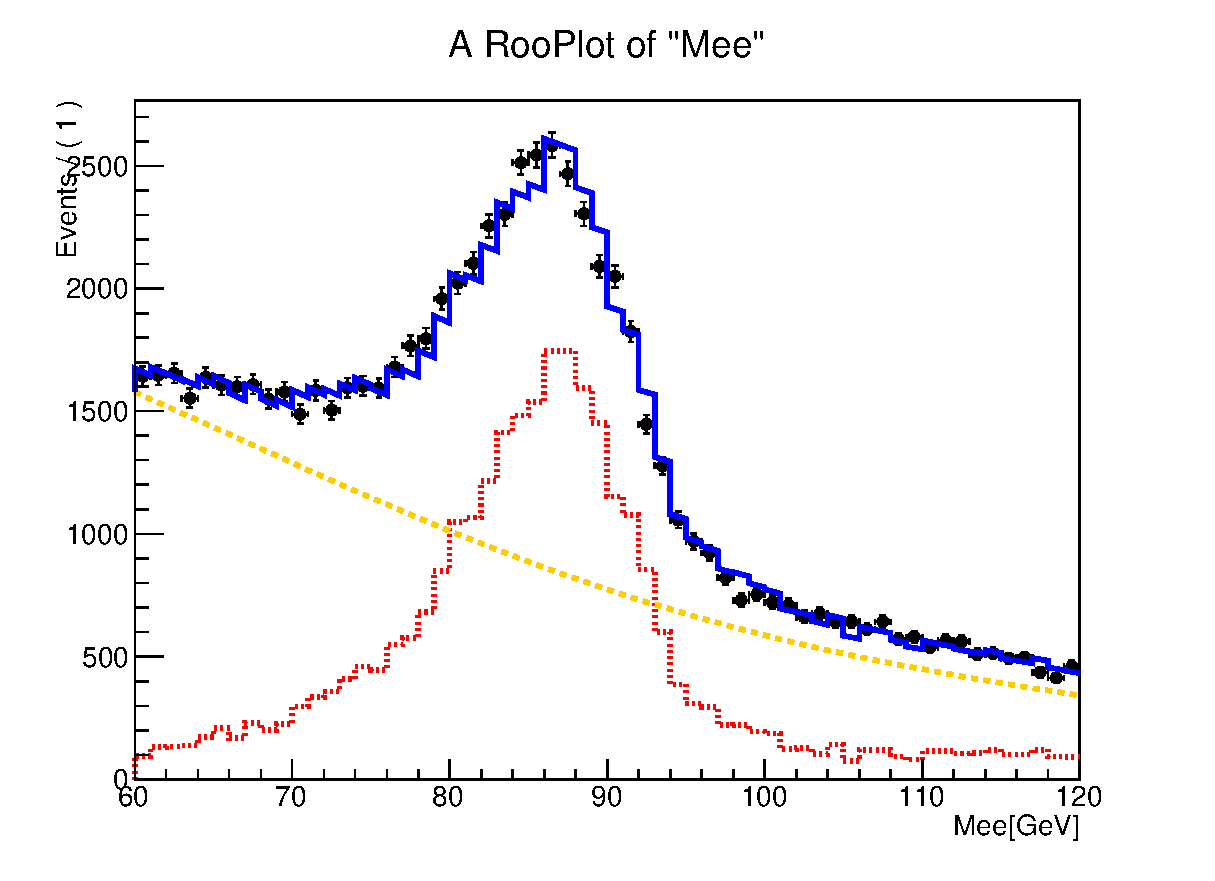
\includegraphics[width=0.5\textwidth]{figures/ChargeMisID/Tot_Polynomial_0_2.eps}
\caption{This plot is polynomial fit for events with first electron's
  $|\eta|$ between [0,0.8] and second electron's $|\eta|$ between
  [1.15,1.60], red line is the \Zee\ signal component, orange
  polynomial is the background component from the fit, black solid
  line is from data sample selected using reversed electron
  identification and isolation cuts and the blue line is the fit.}
\label{fig:Polynomialac}
\end{figure} 

%From Figure.~\ref{fig:Polynomialac}, we can see that the polynomial fit is successful and in this way we can get clean background $ee$ invariant mass histograms for different bins and we use the 4th order polynomial functions obtained here as background templates. 
Thus we can use template fit to estimate the amount of background in
data with the signal template and background template. The signal
template is shown in Fig.~\ref{fig:Signal} and the template fit for
events whose first electron's $|\eta|$ between [0,0.8] and second
electron's $|\eta|$ between [1.15,1.60] is presented in
Fig.~\ref{fig:Template fit}.
\begin{figure}[htp]
  \begin{minipage}[t]{0.5\linewidth}
  \centering
  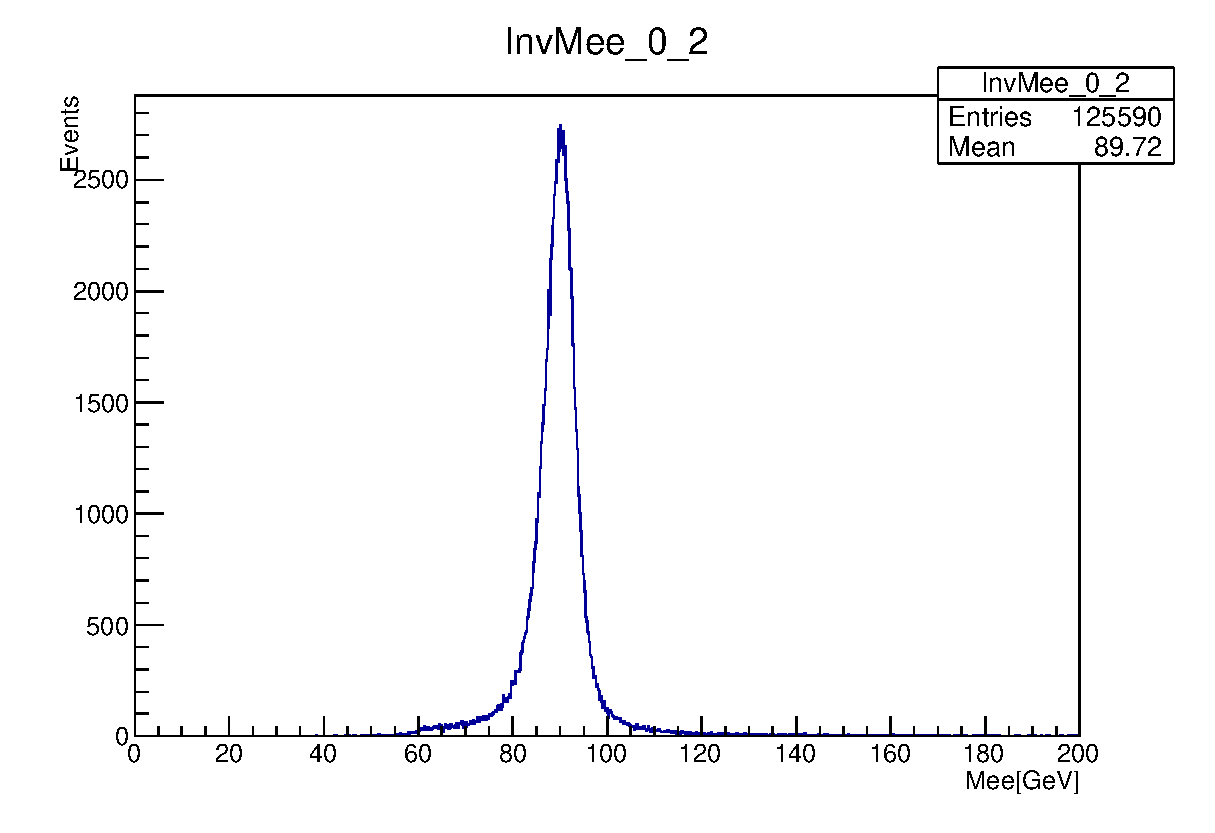
\includegraphics[width=\columnwidth]{figures/ChargeMisID/MergeEt_Ntot_Zee02.eps}
  \caption{Signal $ee$ invariant mass distribution}
  \label{fig:Signal}
  \end{minipage}
  \begin{minipage}[t]{0.5\linewidth}
  \centering
  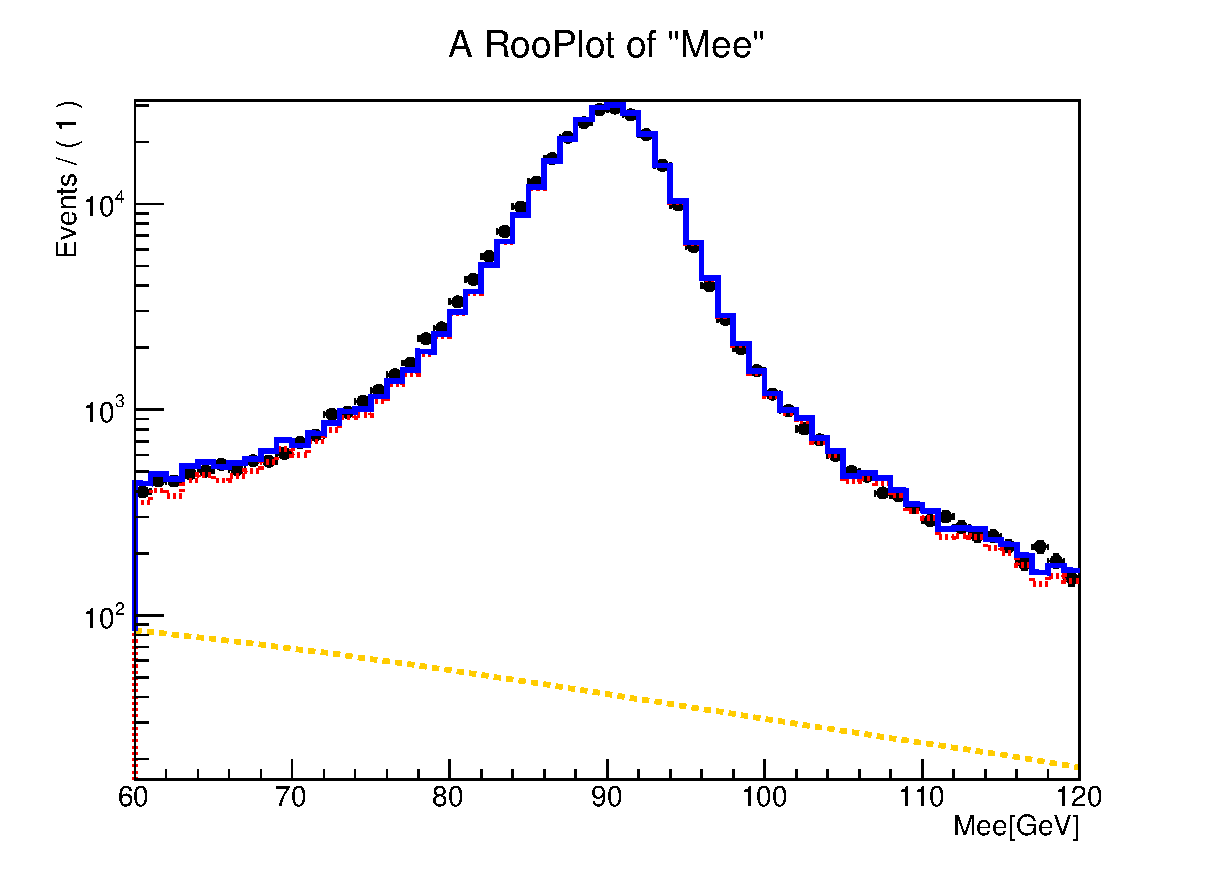
\includegraphics[width=\columnwidth]{figures/ChargeMisID/Tot_Template_0_2.eps}
  \caption{This plot is template fit for events with first electron's $|\eta|$ between[0,0.8] and second electron's $|\eta|$ between[1.15,1.60], red line is the \Zee\ signal component, orange polynomial is the background component from the fit, black solid line is from data sample and the blue line is the fit.}
  \label{fig:Template fit}
  \end{minipage}
\end{figure}  

With template fit, we can get the signal purities in different bins, and we use the signal purities here to estimate the background amount. We need the signal purity of both total events and same sign events to calculate another set of mis-charge rates without background contamination. The numbers presented in Table~\ref{tab:fSig Ntot} and Table~\ref{tab:fSig error Ntot} are the signal purity and statistic errors of signal purities for total events. 
\begin{table}
\footnotesize
\centering
\begin{tabular}{c|c|c|c|c|c|c|c|c|c}
  \hline
   &[0,0.8] &[0.8,1.15] &[1.15,1.60] &[1.60,1.80] &[1.80,2.0] &[2.0,2.20] &[2.20,2.30] &[2.30,2.40] &[2.40,2.50] \\
  \hline
  [0,0.8]  &0.9951 &0.9966 &0.9945 &0.9956 &0.9953 &0.9924 &0.9961 &0.9898 &0.9893 \\
  \hline
  [0.8,1.15]  &0.996 &0.9982 &0.9933 &0.9887 &0.9939 &0.9953 &0.992 &0.9935 &0.972 \\
  \hline
  [1.15,1.60]  &0.9904 &0.9895 &0.9892 &0.9885 &0.9895 &0.9942 &0.9875 &0.9912 &0.9802 \\
  \hline
  [1.60,1.80] &0.9794 &0.9766 &0.9787 &0.9799 &0.9828 &0.9822 &0.9775 &0.9674 &0.9534 \\
  \hline
  [1.80,2.0]  &0.9914 &0.992 &0.994 &0.9878 &0.9927 &0.9906 &0.9906 &0.9912 &0.9546 \\
  \hline
  [2.0,2.20] &0.9934 &0.9978 &0.9833 &0.9872 &0.9936 &0.9847 &0.9837 &0.9717 &0.9776 \\
  \hline
  [2.20,2.30] &0.998 &0.9874 &0.9901 &0.9743 &0.992 &0.9874 &0.9813 &0.9835 &0.9509 \\
  \hline
  [2.30,2.40] &0.9891 &0.9883 &0.9825 &0.9734 &0.9916 &0.9846 &0.9698 &0.9643 &0.9739 \\
  \hline
  [2.40,2.50] &0.9774 &0.9636 &0.9794 &0.9703 &0.9766 &0.9805 &0.9804 &0.9509 &0.9211 \\
  \hline
\end{tabular}
\caption{Signal purity for total events, different rows stand for different $|\eta|$ bins of the sub-leading electron in the event, and different columns stand for different $|\eta|$ bins of the leading electrons in the event.} 
\label{tab:fSig Ntot}
\end{table}
 
\begin{table}
\footnotesize
\centering
\begin{tabular}{c|c|c|c|c|c|c|c|c|c}
  \hline
   &[0,0.8] &[0.8,1.15] &[1.15,1.60] &[1.60,1.80] &[1.80,2.0] &[2.0,2.20] &[2.20,2.30] &[2.30,2.40] &[2.40,2.50] \\
  \hline
  [0,0.8] &0.0004 &0.0006 &0.0008 &0.0011 &0.0012 &0.0011 &0.0016 &0.0019 &0.0028\\
  \hline
  [0.8,1.15] &0.0006 &0.0010 &0.0013 &0.0020 &0.0021 &0.0019 &0.0029 &0.0030 &0.0038 \\
  \hline
  [1.15,1.60] &0.0008 &0.0013 &0.0016 &0.0023 &0.0021 &0.0020 &0.0027 &0.0031 &0.0038 \\
  \hline
  [1.60,1.80] &0.0013 &0.0021 &0.0022 &0.0030 &0.0027 &0.0027 &0.0036 &0.0043 &0.0058 \\
  \hline
  [1.80,2.0] &0.0012 &0.0019 &0.0021 &0.0026 &0.0025 &0.0022 &0.0024 &0.0044 &0.0055 \\
  \hline
  [2.0,2.20] &0.0013 &0.0016 &0.0021 &0.0024 &0.0025 &0.0023 &0.0035 &0.0035 &0.0051 \\
  \hline
  [2.20,2.30] &0.0017 &0.0029 &0.0029 &0.0037 &0.0045 &0.0029 &0.0058 &0.0044 &0.0076 \\
  \hline
  [2.30,2.40] &0.0019 &0.0030 &0.0032 &0.0039 &0.0031 &0.0029 &0.0045 &0.0046 &0.0061 \\
  \hline
  [2.40,2.50] &0.0031 &0.0048 &0.0045 &0.0051 &0.0046 &0.0040 &0.0061 &0.0072 &0.0118 \\
  \hline
\end{tabular}
\caption{Statistical uncertainties of the purities listed in Table~\ref{tab:fSig Ntot}}
\label{tab:fSig error Ntot}
\end{table}

For the same-sign events, the same method is used to estimate the
background contribution, but with all events merged because the
statistics is very limited in the data sample. The global polynomial
fit for same sign events is shown in Fig.~\ref{fig:Global Polynomial}
and the global template fit for same sign events is shown in
Fig.~\ref{fig:Global Template}.
\begin{figure}[htp]
  \begin{minipage}[t]{0.5\linewidth}
  \centering
  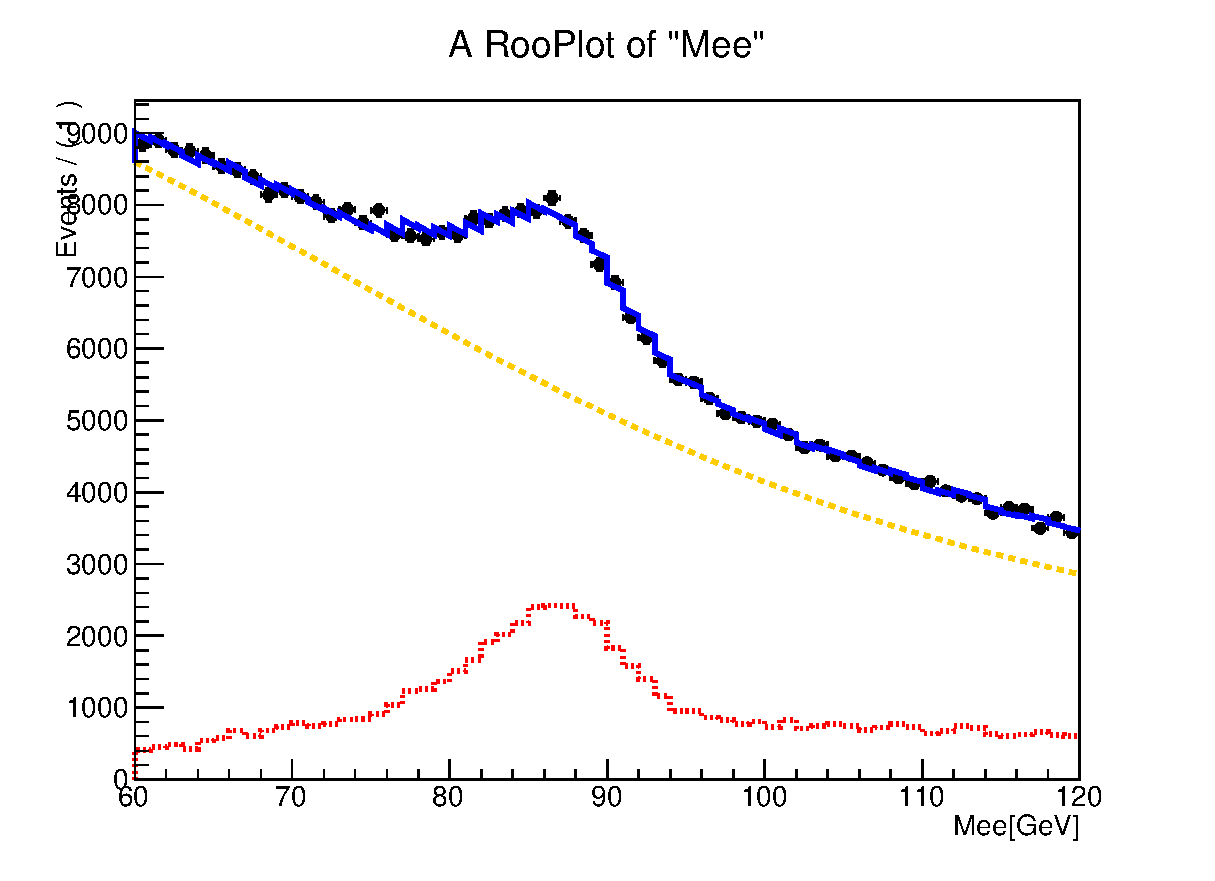
\includegraphics[width=\columnwidth]{figures/ChargeMisID/SS_Polynomial.eps}
  \caption{Global polynomial fit for total events}
  \label{fig:Global Polynomial}
  \end{minipage}
  \begin{minipage}[t]{0.5\linewidth}
  \centering
  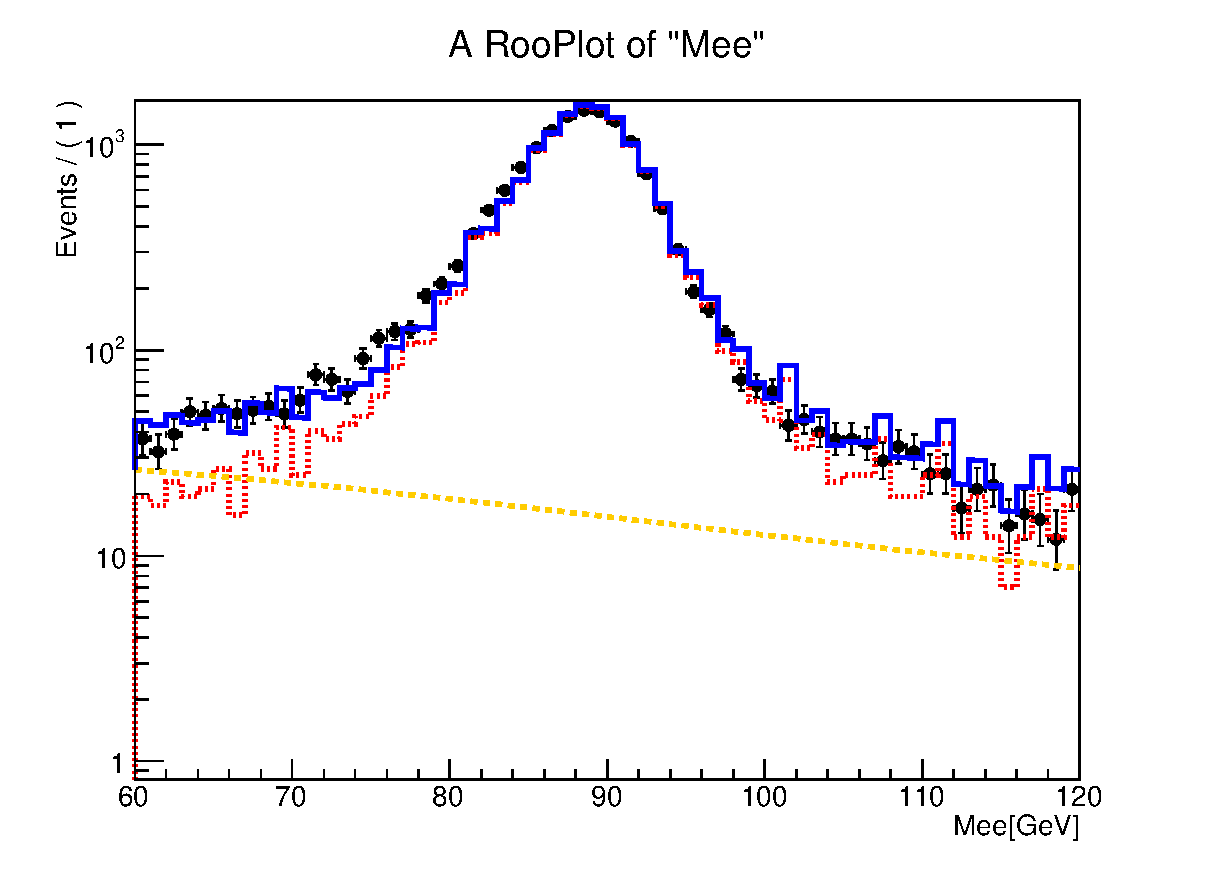
\includegraphics[width=\columnwidth]{figures/ChargeMisID/SS_Template.eps}
  \caption{Global template fit for same sign events.}
  \label{fig:Global Template}
  \end{minipage}
\end{figure} 

Using the template fitting, we obtain the global purity of same sign
events as 0.9372$\pm$0.0042(stat), and the global purity of opposite
sign events as 0.9921$\pm$ 0.0013(stat). The ratio of signal purities
is 0.9447 and is assumed to be independent of different $\eta$
bins. For each $\eta_1 - \eta_2$ bin, we scale the purity of opposite
sign events with this ratio to obtain an estimation of the purity of
the same sign events.

\begin{table}
\footnotesize
\centering
\begin{tabular}{c|c|c|c|c|c|c|c|c|c}
  \hline
   &[0,0.8] &[0.8,1.15] &[1.15,1.60] &[1.60,1.80] &[1.80,2.0] &[2.0,2.20] &[2.20,2.30] &[2.30,2.40] &[2.40,2.50] \\
  \hline
  [0,0.8] &0.9958 &0.997 &0.9947 &0.9958 &0.9951 &0.9924 &0.9968 &0.9871 &0.9863 \\
  \hline
  [0.8,1.15] &0.9964 &0.9982 &0.9937 &0.9882 &0.9937 &0.9951 &0.9924 &0.993 &0.9707 \\
  \hline
  [1.15,1.60] &0.9904 &0.9896 &0.9889 &0.9883 &0.9899 &0.9938 &0.988 &0.9913 &0.9792 \\
  \hline
  [1.60,1.80] &0.9786 &0.9765 &0.9784 &0.9771 &0.9811 &0.9815 &0.9753 &0.9638 &0.9483 \\
  \hline
  [1.80,2.0] &0.9907 &0.9918 &0.9944 &0.9876 &0.9921 &0.9911 &0.9893 &0.9924 &0.9527 \\
  \hline
  [2.0,2.20] &0.9938 &0.9979 &0.9826 &0.9882 &0.9934 &0.9815 &0.9844 &0.9735 &0.9777 \\
  \hline
  [2.20,2.30] &0.9982 &0.9872 &0.9903 &0.9711 &0.9921 &0.987 &0.9841 &0.9779 &0.9391 \\
  \hline
  [2.30,2.40] &0.9898 &0.9848 &0.9826 &0.9719 &0.9897 &0.984 &0.9667 &0.9562 &0.9637 \\
  \hline
  [2.40,2.50] &0.9775 &0.9656 &0.9784 &0.9628 &0.974 &0.9783 &0.9771 &0.9513 &0.9226 \\
  \hline
\end{tabular}
\caption{Signal purity of opposite sign events, different rows stand
  for different $|\eta|$ bins of the sub-leading electron in the
  event, and different columns stand for different $|\eta|$ bins of
  the leading electrons in the event.}
\label{tab:fSig Nos}
\end{table}

\begin{table}
\footnotesize
\centering
\begin{tabular}{c|c|c|c|c|c|c|c|c|c}
  \hline
   &[0,0.8] &[0.8,1.15] &[1.15,1.60] &[1.60,1.80] &[1.80,2.0] &[2.0,2.20] &[2.20,2.30] &[2.30,2.40] &[2.40,2.50] \\
  \hline
  [0,0.8] &0.0003 &0.0006 &0.0008 &0.0011 &0.0013 &0.0012 &0.0017 &0.0022 &0.0032 \\
  \hline
  [0.8,1.15] &0.0006 &0.0010 &0.0013 &0.0020 &0.0021 &0.0018 &0.0029 &0.0032 &0.0039 \\
  \hline
  [1.15,1.60] &0.0008 &0.0014 &0.0016 &0.0023 &0.0021 &0.0020 &0.0028 &0.0032 &0.0040 \\
  \hline
  [1.60,1.80] &0.0013 &0.0021 &0.0022 &0.0031 &0.0029 &0.0027 &0.0042 &0.0047 &0.0063 \\
  \hline
  [1.80,2.0] &0.0012 &0.0020 &0.0022 &0.0027 &0.0026 &0.0023 &0.0028 &0.0044 &0.0057 \\
  \hline
  [2.0,2.20] &0.0012 &0.0020 &0.0021 &0.0022 &0.0026 &0.0031 &0.0034 &0.0035 &0.0055 \\
  \hline
  [2.20,2.30] &0.0017 &0.0030 &0.0030 &0.0040 &0.0045 &0.0031 &0.0058 &0.0048 &0.0075 \\
  \hline
  [2.30,2.40] &0.0020 &0.0027 &0.0032 &0.0041 &0.0033 &0.0029 &0.0050 &0.0052 &0.0069 \\
  \hline
  [2.40,2.50] &0.0031 &0.0048 &0.0045 &0.0053 &0.0050 &0.0044 &0.0065 &0.0074 &0.0122 \\
  \hline
\end{tabular}
\caption{Statistical uncertainties of the purities listed in
  Table~\ref{tab:fSig Nos}.}
\label{tab:fSig error Nos}
\end{table}

\begin{table}
\footnotesize
\centering
\begin{tabular}{c|c|c|c|c|c|c|c|c|c}
  \hline
   &[0,0.8] &[0.8,1.15] &[1.15,1.60] &[1.60,1.80] &[1.80,2.0] &[2.0,2.20] &[2.20,2.30] &[2.30,2.40] &[2.40,2.50] \\
  \hline
  [0,0.8] &0.9407 &0.9419 &0.9397 &0.9408 &0.9401 &0.9375 &0.9417 &0.9325 &0.9317 \\
  \hline
  [0.8,1.15] &0.9413 &0.943 &0.9387 &0.9335 &0.9387 &0.9401 &0.9375 &0.9381 &0.917 \\
  \hline
  [1.15,1.60] &0.9357 &0.9349 &0.9342 &0.9337 &0.9352 &0.9389 &0.9334 &0.9365 &0.9251 \\
  \hline
  [1.60,1.80] &0.9245 &0.9225 &0.9243 &0.9231 &0.9268 &0.9272 &0.9214 &0.9105 &0.8958 \\
  \hline
  [1.80,2.0] &0.9359 &0.937 &0.9394 &0.933 &0.9372 &0.9363 &0.9346 &0.9375 &0.9 \\
  \hline
  [2.0,2.20] &0.9389 &0.9427 &0.9283 &0.9336 &0.9384 &0.9273 &0.93 &0.9197 &0.9237 \\
  \hline
  [2.20,2.30] &0.943 &0.9326 &0.9355 &0.9174 &0.9372 &0.9325 &0.9297 &0.9238 &0.8872 \\
  \hline
  [2.30,2.40] &0.935 &0.9304 &0.9283 &0.9181 &0.935 &0.9296 &0.9133 &0.9033 &0.9104 \\
  \hline
  [2.40,2.50] &0.9235 &0.9122 &0.9243 &0.9095 &0.9202 &0.9242 &0.9231 &0.8987 &0.8716 \\
  \hline
\end{tabular}
\caption{Signal purity of same sign events, different rows stand for
  different $|\eta|$ bins of the sub-leading electron in the event,
  and different columns stand for different $|\eta|$ bins of the
  leading electrons in the event.}
\label{tab:fSig Nss}
\end{table}

\begin{table}
\footnotesize
\centering
\begin{tabular}{c|c|c|c|c|c|c|c|c|c}
  \hline
  &[0,0.8] &[0.8,1.15] &[1.15,1.60] &[1.60,1.80] &[1.80,2.0] &[2.0,2.20] &[2.20,2.30] &[2.30,2.40] &[2.40,2.50] \\
  \hline
  [0,0.8] &0.0003 &0.0006 &0.0007 &0.0011 &0.0012 &0.0011 &0.0016 &0.0021 &0.0031 \\
  \hline
  [0.8,1.15] &0.0005 &0.0009 &0.0012 &0.0019 &0.0020 &0.0017 &0.0028 &0.0031 &0.0037 \\
  \hline
  [1.15,1.60] &0.0007 &0.0013 &0.0015 &0.0022 &0.0019 &0.0019 &0.0027 &0.0030 &0.0038 \\
  \hline
  [1.60,1.80] &0.0012 &0.0020 &0.0021 &0.0030 &0.0027 &0.0025 &0.0040 &0.0044 &0.0059 \\
  \hline
  [1.80,2.0] &0.0012 &0.0019 &0.0020 &0.0025 &0.0024 &0.0021 &0.0026 &0.0042 &0.0054 \\
  \hline
  [2.0,2.20] &0.0012 &0.0019 &0.0020 &0.0021 &0.0024 &0.0029 &0.0032 &0.0033 &0.0052 \\
  \hline
  [2.20,2.30] &0.0016 &0.0029 &0.0028 &0.0038 &0.0042 &0.0030 &0.0055 &0.0045 &0.0071 \\
  \hline
  [2.30,2.40] &0.0019 &0.0025 &0.0030 &0.0039 &0.0031 &0.0028 &0.0047 &0.0049 &0.0066 \\
  \hline
  [2.40,2.50] &0.0029 &0.0046 &0.0043 &0.0050 &0.0047 &0.0041 &0.0061 &0.0070 &0.0116 \\ 
  \hline
\end{tabular}
\caption{Statistical uncertainties of the purities listed in Table~\ref{tab:fSig Nss}}
\label{tab:fSig error Nss}
\end{table}

At this stage, we have signal purity and their statistic errors of
total events and same sign events shown in Table~\ref{tab:fSig Ntot},
Table~\ref{tab:fSig error Ntot}, Table~\ref{tab:fSig Nss},
Table~\ref{tab:fSig error Nss} which are input variables to calculate
mis-charge rates, so we subtract the background contribution for total
events and same sign events in Eq.~(\ref{eq:lnL_chargeMisID}) and
calculate another set of electron mis-charge rates. We take the
difference between rates measured with and without background
subtraction as systematic uncertainty. The background systematic
uncertainty is shown in Table~\ref{tab:Bkg Sys}. The typical size of
this uncertainty is about 5\%.
\begin{table}
\footnotesize
\centering
\begin{tabular}{c|c|c|c|c|c|c|c|c|c}
  \hline
  \backslashbox{\pt[\GeV]}{$|$\eta$|$} &[0,0.8] &[0.8,1.15] &[1.15,1.60] &[1.60,1.80] &[1.80,2.0] &[2.0,2.20] &[2.20,2.30] &[2.30,2.40] &[2.40,2.50] \\ 
  \hline
  [15,30] &8.85 &5.63 &5.75 &5.85 &5.79 &5.64 &5.64 &5.68 &5.49 \\
  \hline
  [30,40] &5.73 &5.71 &5.83 &5.97 &5.75 &5.78 &5.72 &5.81 &5.59 \\
  \hline
  [40,50] &5.76 &5.69 &5.71 &5.71 &5.65 &5.71 &5.62 &5.71 &5.62 \\
  \hline
  [50,60] &5.74 &5.55 &5.64 &5.53 &5.61 &5.65 &5.41 &5.49 &5.65 \\
  \hline
  [60,80] &5.77 &5.57 &5.71 &5.99 &5.59 &5.66 &5.35 &5.53 &5.41 \\
  \hline
  [80,120] &5.79 &5.63 &5.73 &5.71 &5.74 &5.77 &5.36 &5.74 &5.89 \\
  \hline
  [120,1000] &5.76 &5.71 &5.54 &5.76 &5.52 &5.61 &5.73 &5.98 &6.14  \\
  \hline
\end{tabular}
\caption{Numbers here are background systematics over central values
  in percent.}
\label{tab:Bkg Sys}
\end{table} 
 



 



